\documentclass[prl,aps,amsfonts,twocolumn,superscriptaddress,notitlepage,floatfix]{revtex4-1}
% \documentclass{article}
% \usepackage{fullpage}
%\usepackage{showkeys}
\usepackage{amsmath,amssymb}
\usepackage{graphicx}
\usepackage{epsfig, color}
\usepackage{wasysym}
\usepackage{amsfonts}
\usepackage{bm}
\usepackage{enumerate}
\usepackage{bbold}
\usepackage{xcolor}
\usepackage[normalem]{ulem}
\usepackage{cancel}
\usepackage{multibib}
\usepackage{comment}

% supplemental material: supp

\usepackage{mathtools}
\DeclarePairedDelimiter{\ceil}{\lceil}{\rceil}

\usepackage{latexsym}
\usepackage[breaklinks,colorlinks = true,linkcolor = blue,urlcolor=cyan,citecolor=red,linktocpage=true]{hyperref}

\newcommand{\be}{\begin{eqnarray}}
\newcommand{\ee}{\end{eqnarray}}
\newcommand{\bent}{\begin{equation*}}
\newcommand{\eent}{\end{equation*}}

\usepackage{pdfpages} % include appendix
\makeatletter
\AtBeginDocument{\let\LS@rot\@undefined}
\makeatother


%% type setting
\newcommand{\vpd}[0]{\vphantom{\dagger}}
\newcommand{\vps}[0]{\vphantom{*}}
\def\jp{j^{\prime}}

%%% Hilbert space / algebra stuff
\def\ket#1{{|#1\rangle}}
\def\bra#1{{\langle #1 |}}
\newcommand{\ident}[0]{ \mathbb{1}}

\newcommand{\inprod}[2]{ \left\langle #1 \middle| #2 \right\rangle}
\newcommand{\winprod}[2]{ \left\langle ~ #1 ~\middle| ~ #2 ~ \right\rangle}

\newcommand{\expval}[1]{ \left\langle #1 \right\rangle}
\newcommand{\wexpval}[1]{ \left\langle ~ #1  ~ \right\rangle}

\newcommand{\matel}[3]{\left\langle #1 \middle| #2 \middle| #3 \right\rangle}
\newcommand{\wmatel}[3]{\left\langle~#1~\middle|~#2~\middle|~#3~\right\rangle}

\newcommand{\tr}[1]{{\rm tr} \left[ #1 \right]}
\newcommand{\trace}{{\rm tr}}
\newcommand{\com}[2]{\left[ #1, \, #2 \right]}
\newcommand{\acom}[2]{\left\{ #1, \, #2 \right\} }
\newcommand{\abs}[1]{\left| #1 \right|}


%% operators\def\observ{\mathcal{O}}
\def\gate{\mathcal{U}}
\def\Haar{U}
\def\Floq{\mathcal{F}}
\def\evo{\mathcal{W}}
\def\Ham{H}
\def\Tmat{\mathcal{T}}
\def\Tgate{T}
\def\observ{\mathcal{O}}

% times
\def\tth{t^{\vpd}_{\rm Th}}
\def\theis{t^{\vpd}_{\rm Heis}}

%dimensions
\def\Hdim{\mathcal{D}}
\def\Ldim{q}
\def\ancilla{d}

% other
\def\disp{\varepsilon}
\def\gap{\Delta}
\def\charge{\mathfrak{q}}
\def\totcharge{Q}
\def\Corr{\mathcal{C}}
\def\numsec{\mathcal{N}}

\newcommand\particle{{\color{black}\bullet}\mathllap{\circ}}
\newcommand\hole{\circ}



%%% Operator space  stuff
\newcommand{\opbra}[1]{\left( #1 \right|}
\newcommand{\wopbra}[1]{\left( \, #1 \, \right|}
\newcommand{\opket}[1]{\left| #1 \right)}
\newcommand{\wopket}[1]{\left| \, #1 \, \right)}

\newcommand{\opinprod}[2]{\left( #1 \middle| #2 \right)}
\newcommand{\wopinprod}[2]{\left( \, #1 \, \middle| \, #2 \, \right)}

\newcommand{\opmatel}[3]{\left( #1 \middle| #2 \middle| #3 \right)}
\newcommand{\wopmatel}[3]{\left( \, #1 \, \middle| \, #2 \, \middle| \, #3 \, \right)}

%editing
\newcommand{\brayden}[1]{ { \color{blue} {{#1}}}}
\newcommand{\romain}[1]{ { \color{red} {{#1}}}}
\newcommand{\aaron}[1]{\color{magenta} {{#1}}}





\begin{document}

\title{Subdiffusion and many-body quantum chaos with kinetic constraints}


\author{Hansveer Singh}
\affiliation{Department of Physics, University of Massachusetts, Amherst, Massachusetts 01003, USA}
\author{Brayden A. Ware}
\affiliation{Department of Physics, University of Massachusetts, Amherst, Massachusetts 01003, USA}
\author{Romain Vasseur}
\affiliation{Department of Physics, University of Massachusetts, Amherst, Massachusetts 01003, USA}
\author{Aaron J. Friedman}
\affiliation{Department of Physics and Center for Theory of Quantum Matter, University of Colorado, Boulder, Colorado 80309, USA}
\date{\today}



\begin{abstract}
We investigate the spectral and transport properties of many-body quantum systems with conserved charges and kinetic constraints. Using random unitary circuits, we compute ensemble-averaged spectral form factors and linear-response correlation functions, and find that their characteristic time scales are given by the inverse gap of an effective Hamiltonian---or equivalently, a transfer matrix describing a classical Markov process. Our approach allows us to connect directly the Thouless time, $t^{\vphantom{\dagger}}_{\rm Th}$, determined by the spectral form factor, to transport properties and linear response correlators. 
Using tensor network methods, we determine the dynamical exponent, $z$, for a number of constrained, conserving models. We find universality classes with diffusive, subdiffusive, quasilocalized, and localized dynamics, depending on the severity of the constraints. In particular, we show that quantum systems with ``Fredkin'' constraints exhibit anomalous  transport with dynamical exponent $z \simeq 8/3$. 


\end{abstract}



\maketitle



\noindent \emph{Introduction.---}\,
Recent years have seen substantial progress in understanding how isolated quantum systems thermalize under their own dynamics.~
The eigenstate thermalization hypothesis (ETH) \cite{ETH1,ETH2} proposes that entanglement between subsystems allows for local equilibration: Generic unitary evolution scrambles local quantum information into highly nonlocal degrees of freedom, which are inaccessible to local observables. Early tests of ETH~\cite{PhysRevLett.98.050405,Rigol2008kq,santos2010onset,borgonovi2016quantum,Rigol} relied on 
small scale numerics and extensions of integrable models, which are fine tuned; understanding the universal aspects of quantum chaotic dynamics requires a more general approach.


A hallmark of chaotic systems is that they dynamically forget as much information about their past as symmetries allow. Hence, the salient features of chaotic systems are well captured by replacing the microscopic model with a random matrix with the same symmetries. Random unitary circuits (RUCs) invoke the potency of random matrix theory (RMT) while also introducing spatial locality, with the system evolved by a brickwork ``circuit'' of $\ell$-site gates \cite{YoshidaCBD,ProsenRMTChaosPRX,NahumRUC1,NahumOperator,RUCNCTibor,CiracRUFC,CDLC1,Kos_2021,U1FRUC}. RUCs are fully generic, and their study has elucidated the universal dynamics of chaotic quantum systems: Entanglement grows linearly until saturating to a volume law, with fluctuations in the KPZ universality class \cite{NahumRUC1}; operator fronts (and out-of-time-ordered correlation functions) propagate ballistically and broaden diffusively \cite{NahumOperator,RUCNCTibor,CDLC1}, etc. 

However, these RUCs are designed to be featureless; an interesting question is how these properties change as one reintroduces other physical ingredients, such as symmetries. With conserved charges, one can consider transport; for typical $U(1)$ symmetry, one expects conserved charges to diffuse \cite{RUCconTibor,RUCconVedika,ShenkerRMT,U1FRUC}. Operators that overlap with conserved quantities are expected to have slower dynamics, dominated by hydrodynamic modes. It is also interesting to study dynamics %in the presence of 
with more complicated symmetries or constraints~\cite{Valado_2016,PhysRevB.94.235122, PhysRevLett.121.085701, GopalakrishnanAutomata_2018, Lan_2018,Everest_2016,QuantumEast2020,Scherg_2021,PhysRevLett.122.250602,PhysRevResearch.2.033020,Huang_2020}. Fractons, e.g., are excitations in systems with charge and dipole conservation, which are constrained to move in pairs only \cite{SagarFracton1,SagarFracton2}. This higher-order symmetry can also be viewed as a \emph{constraint}; recent studies of fractons in the contexts of RUCs and hydrodynamics have found evidence for subdiffusion, with dynamical exponent $z=2(m+1)$, where $m$ is the highest conserved moment of charge~\cite{FractonSubdiffusionDim,FractonHydro,PhysRevLett.125.245303,morningstarKineticallyConstrainedFreezing2020,FractonSubdiffusion,glorioso2021breakdown,SanjayAmosFracton}.



In this Letter we analyze the general consequences of kinetic constraints on charge-conserving many-body quantum dynamics in one dimension. Kinetic constraints restrict the local rearrangements of charges and have been intensely studied as models of classical systems with glassy dynamics \cite{Valado_2016,QuantumEast2020,Scherg_2021,Lan_2018,Everest_2016,garrahan2010kinetically,GarrahanLectures,RitortKCM,KCMRydberg}. Depending on the %local geometry of the 
locally forbidden rearrangements, adding constraints may anomalously slow down or completely freeze the process of thermalization. Using variations of RUCs, we probe how imposing constraints on generic quantum systems leads to new universality classes with slow dynamics. Using Floquet random circuits, in the limit of large on-site Hilbert space, we relate the scaling of the many-body Thouless time---the time scale for a system to show RMT spectral rigidity---with system size~\cite{CDLC1,CDLC2,bertini2018exact,ShenkerRMT,ShenkerRMT,FyodorovMirlin,CiracRUFC,U1FRUC,SwingleSFFHydro,SwingleSFFSSB,Kos_2021} to the inverse gap of the transfer matrix of a stochastic classical model; or equivalently, of an effective Hamiltonian, which lies at a Rokhsar-Kivelson (RK) point \cite{RK,SanjayAmosFracton,U1FRUC}. We show that the same %effective Hamiltonian 
transfer matrix also controls the dynamics of linear response correlators, providing a general relation between the Thouless time and transport \cite{ShenkerRMT}. Depending on the severity of the model's constraints, we find %models with 
diffusive, subdiffusive, quasilocalized, and localized dynamics, and identify a new universality class of constrained $z \simeq 8/3$ ``Fredkin'' systems \cite{FredkinEntanglement,Korepin2016fredkin,Korepin2017fredkin,ChenFredkin2017,ChenFredkin2017a,Zhang2017fredkin,Udagawa2017fredkin,FredkinFragmentScar,ChenFredkin2020}% characterized by a
%, with dynamical exponent $z \simeq 8/3$.
.

\noindent \emph{Spectral rigidity and transport correlators.---}\, A useful indicator of quantum chaos is \emph{level repulsion} \cite{ETH1,ETH2,ShenkerRMT}, characterized by an RMT distribution of the eigenvalues of the evolution operator~\cite{ShenkerRMT,ShenkerRMT,ProsenRMTChaosPRX,SwingleSFFHydro,CDLC1,CDLC2,U1FRUC,Kos_2021}. Periodically driven (Floquet) RUCs~\cite{CDLC1,CDLC2,CiracRUFC,U1FRUC}, afford such a spectrum, as time evolution follows from the Floquet unitary, $\Floq$, that evolves the system by one time step. For Hamiltonian or Floquet systems, it is convenient to measure the ratio of consecutive energy gaps (the ``$r$ ratio'') \cite{rratio}; another robust probe of spectral rigidity is the two-point spectral form factor (SFF)  \cite{bertini2018exact,FyodorovMirlin,CDLC1,CDLC2,U1FRUC,ShenkerRMT,ShenkerRMT,SwingleSFFHydro,SwingleSFFSSB,Kos_2021}, 
\be \label{eq:Ktdef}
K(t) \equiv \sum\limits_{m,n = 1}^{\Hdim} \, \overline{\, e^{\mathbf{i} \left( \theta_m - \theta_n \right) t } }\, = \overline{\, \left| \trace [ \, \Floq^t \, ] \right|^2 \,}~~,~~~
\ee
where $\{\theta^{\,}_m\}$ are the eigenphases of $\Floq$, $\Hdim=\Ldim^L$ with $L$ the number of sites and $\Ldim$ states per site, and the overline denotes averaging over an ensemble of statistically similar systems. In the limit $\Ldim \to \infty$, RUCs reproduce the spectral properties of nonlocal random matrix models \cite{BnB,CDLC1}: $K(t) = t$ for $0 < t < \theis = \Hdim$, the Heisenberg time, and $K(t) = \Hdim$ for $t>\theis$. In this limit, thermalization---characterized by a linear ramp $K = t$---is instantaneous. 




Away from this limit, one expects an initial overshoot of the linear ramp until interactions thermalize the system \cite{CDLC2,SwingleSFFHydro}. A noninteracting Floquet RUC has $K = t^L$; one can imagine divvying the system into weakly interacting 
blocks of size $\xi (t)$, so that $K(t) \sim t^{L/\xi (t)}$, with $\xi (0) \sim 1$. Under time evolution, interactions lead $\xi (t)$ to grow, saturating to $\xi  (t) = L$ for $t \geq \tth$, so that $K(t) = t$ \cite{ShenkerRMT,CDLC1,ProsenRMTChaosPRX,bertini2018exact,U1FRUC}. The Thouless time, $\tth$---in analogy to single-particle disordered wires \cite{Thouless74,ThoulessThinWire}---is the time it takes for a chaotic system to thermalize fully, signaled by a linear ramp, $K(t) = t$. 

One can also observe delayed thermalization even for $\Ldim \to \infty$ with conserved charges \cite{ShenkerRMT,U1FRUC}. Symmetries (and constraints) lead to independent sectors of $\Floq$ whose eigenvalues do not repel; thus, a chaotic system with $\numsec$ independent sectors will have $K(t) = \numsec \, t$ after thermalizing \cite{U1FRUC}. Ref.~\citenum{U1FRUC} provides a recipe for computing the SFF in the presence of symmetries, mapping $K(t)$ to a classical Markov process, itself equivalent to a quantum Hamiltonian at an RK point~\cite{RK,U1FRUC,SanjayAmosFracton}. Study of the corresponding classical lattice gas reveals that diffusion of the $U(1)$ conserved charge delays thermalization, with $K(t) \to \numsec \, t$ for $t \gtrsim \tth \sim L^2$. Slower, subdiffusive scalings of $\tth$ have also been observed in systems with dipole-moment conservation~\cite{SanjayAmosFracton}.


In this work, we investigate the effect of constraints and symmetries on thermalization by studying the SFF and linear response (connected) transport correlators,
%
\be \label{eq:Cdef}
\Corr (x,t) \, = \, \expval{\, \charge (x,t) \, \charge (0,0) \, }^{\,}_{c} ~~,~~
\ee
% 
with $\charge (x)$ the local charge density, $\totcharge =\int dx \, \charge (x)$ the conserved $U(1)$ charge, and $\expval{ \, \dots \, } \,  = \, \Hdim^{-1} \, \tr{\, \dots \,}$, the equilibrium average at infinite temperature \footnote{Subtraction of the disconnected part is implied. Connected correlators in the spin and particle language are identical up to a factor of four.}. We provide a recipe for computing the structure factor~\eqref{eq:Cdef} for arbitrary $\Ldim$, and the SFF \eqref{eq:Ktdef} for $\Ldim \to \infty$ in generic, quantum chaotic models, using the machinery of RUCs. We show that the important physics of \emph{both} quantities is controlled by the low energy properties of the \emph{same} transfer matrix, $\Tmat$, which also describes a discrete-time Markov process with the same conservation laws and constraints~\footnote{Such a direct connection between the spectral form factor and two-point correlators was first suggested in Ref.~\citenum{ShenkerRMT}.}. We can also view $\Tmat^{t} \approx e^{- t \, \Ham^{\,}_{\rm RK}}$, where $\Ham^{\,}_{\rm RK}$ lies at an unfrustrated RK point~\cite{RK,U1FRUC,SanjayAmosFracton}. Within a fixed charge sector, the gap of $\Tmat$ (or $\Ham^{\,}_{\rm RK}$) scales as $\gap \sim L^{-z}$; its inverse is the Thouless time, $\tth \sim L^z$, the time required for information to relax throughout the system. The same dynamical exponent controls transport properties from~\eqref{eq:Cdef}, and we find a universal scaling form $ \Corr (x,t) \sim t^{-1/z} f(x/t^{1/z})$, with $z=2$ and $f(\cdot)$ Gaussian for diffusive systems, and $z>2$ for subdiffusive systems.

\begin{figure}[t!]
\centering
	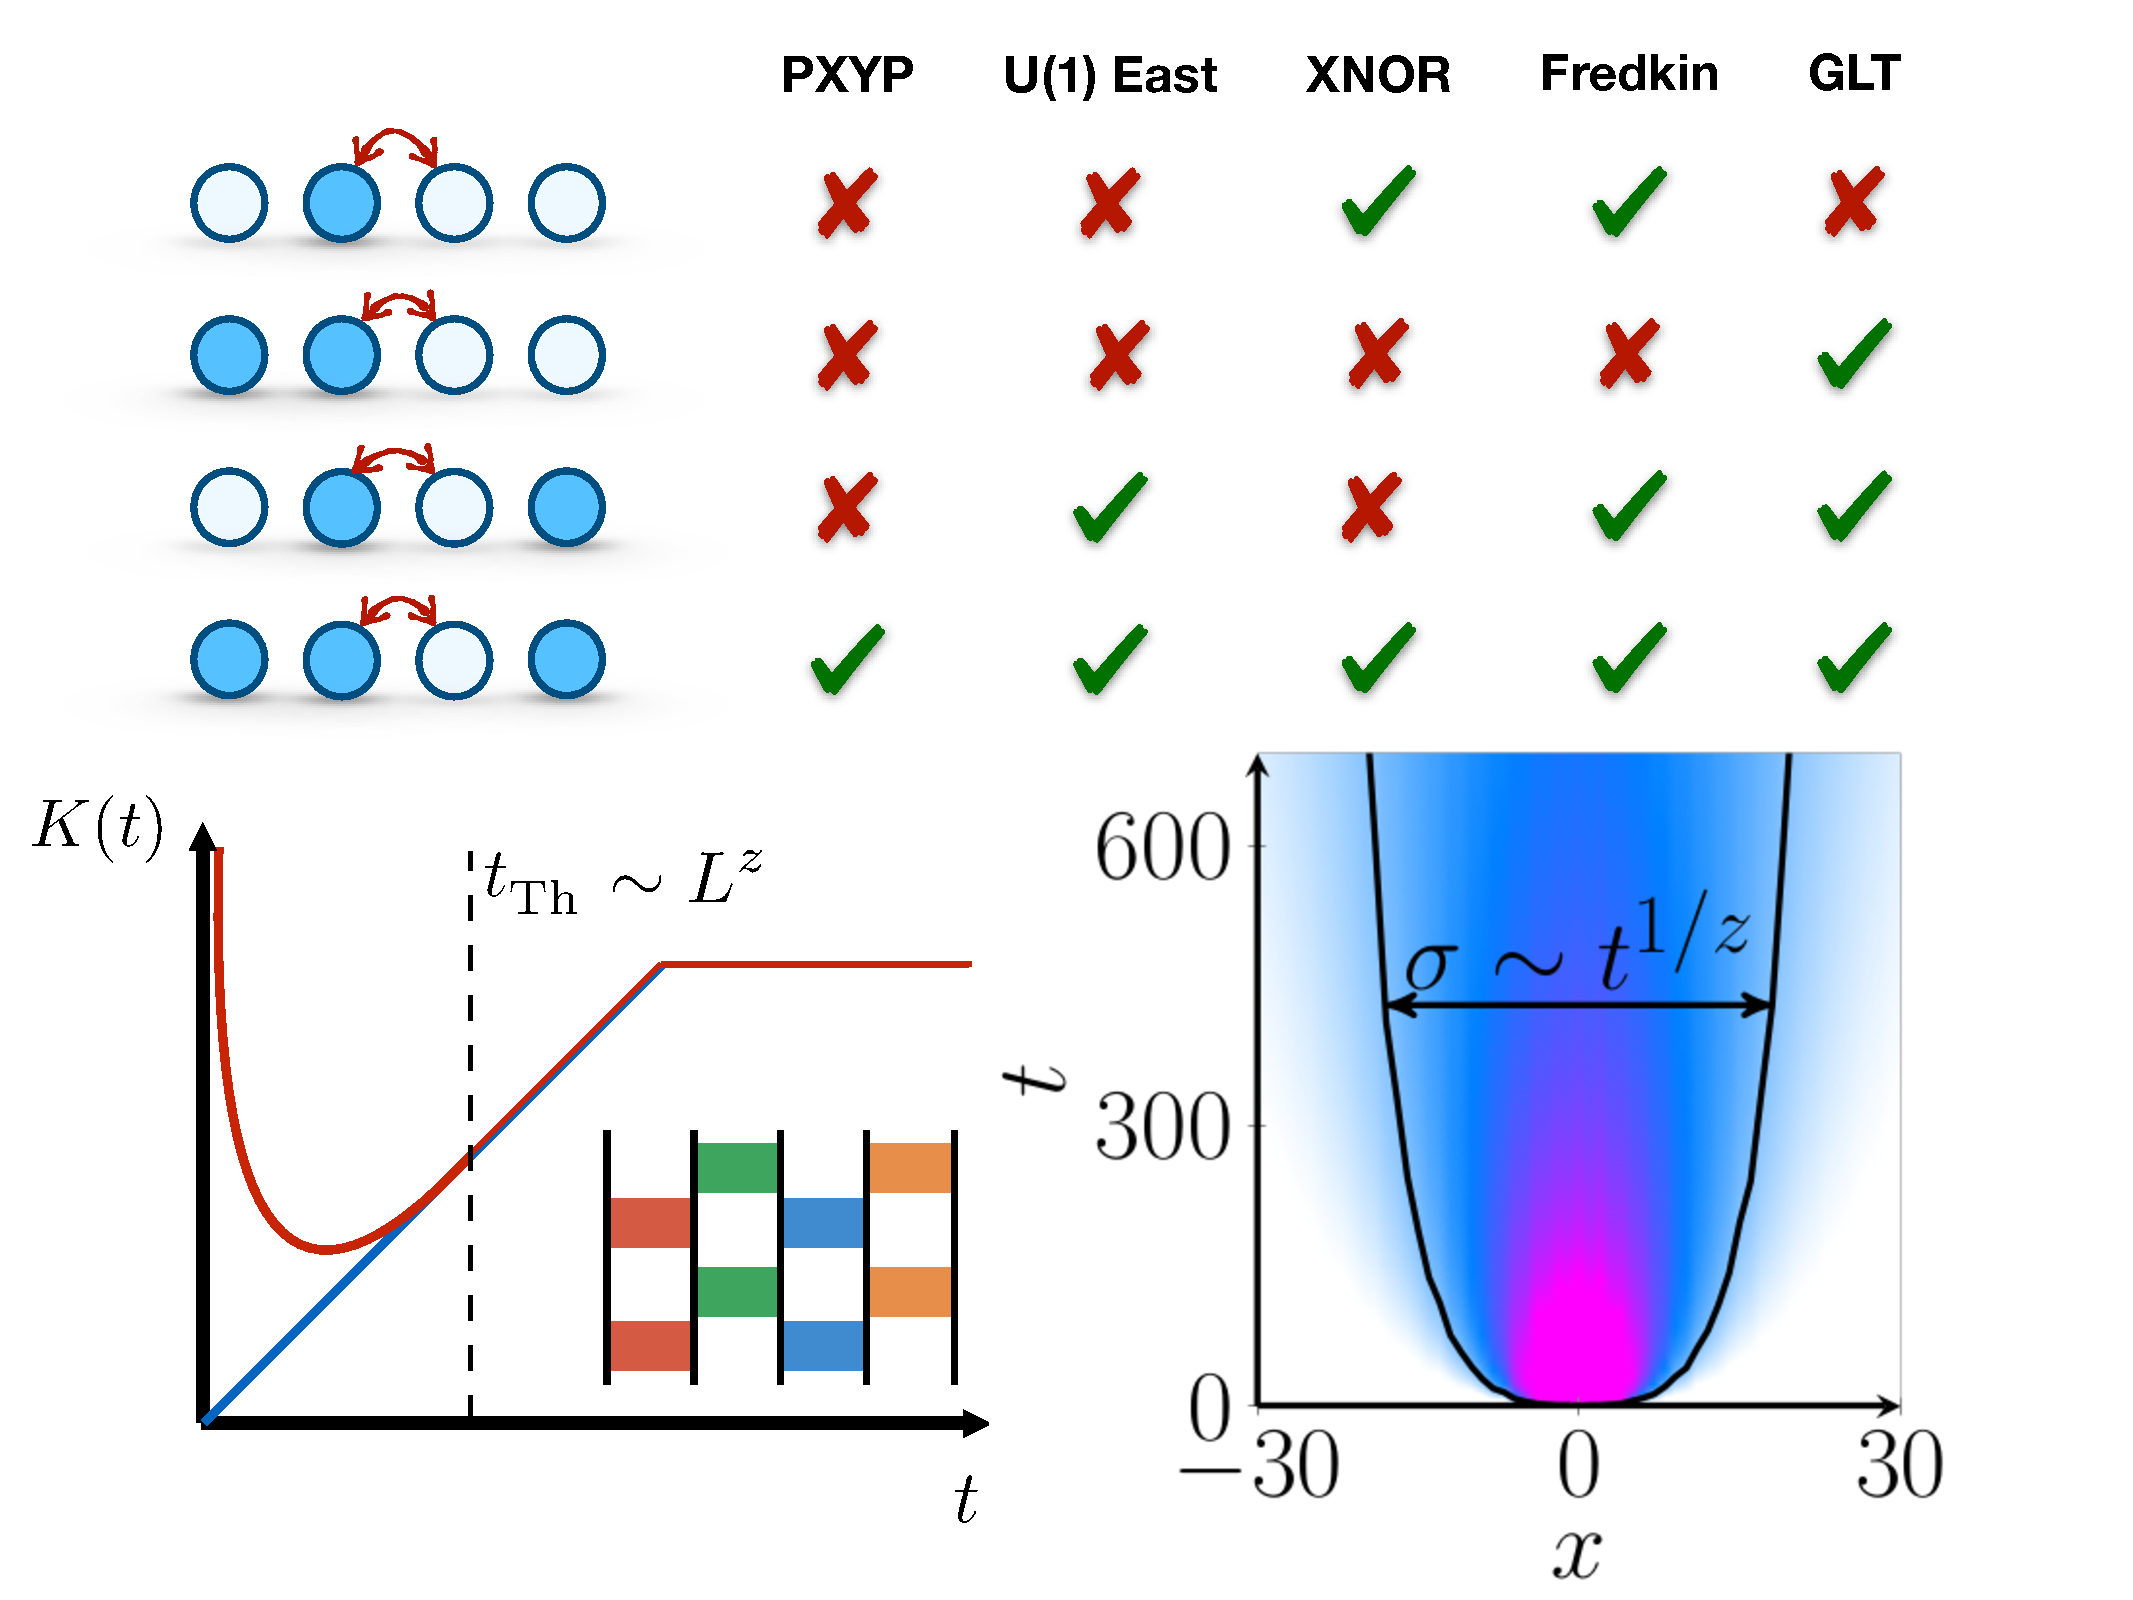
\includegraphics[width = 0.95\columnwidth]{Fig1.pdf} 
	\caption{
	{\bf Models and setup.} {\it Top}:~Cartoon depiction of the allowed dynamical moves for the five models presented; $\particle$ indicates a particle and $\hole$ denotes a hole. {\it Bottom Left}:~Cartoon sketch of the spectral form factor for a generic chaotic system (red) and the RMT prediction (blue); the linear ramp regime ($K(t) = \numsec t$) sets in for $t \gtrsim t^{\,}_{\rm Th}$, the Thouless time, which scales as $L^z$. {\it Bottom Right}:~Heat map of the structure factor (charge two-point function), shown here for Fredkin RUCs, with the variance used to extract $z$, the dynamical critical exponent ($z \simeq 8/3$ for Fredkin constraints).
	\label{fig1} }
\end{figure}


\noindent \emph{Models.---}\, We consider several constrained models acting on a chain of $L$ qubits ($\Ldim=2$) which may be occupied ($\particle$) or empty ($\hole$), with a $U(1)$ conserved charge corresponding to particle number. A cartoon of the allowed dynamical moves is given in Fig.~\ref{fig1}: Essentially, particles are allowed to hop if the neighboring sites are appropriately occupied/unoccupied. Time evolution is generated by a circuit of gates with the general form
\be \label{eq:GateForm} \gate^{\,}_r \, = \, \sum\limits_{\alpha} \, P^{\,}_{r,\alpha} \, \Haar^{\,}_{r,\alpha} \, P^{\,}_{r,\alpha} \, + \, \sum\limits_{\beta} \, P^{\,}_{r,\beta}~~,~~\ee
where $\alpha$ labels constraint-satisfying configurations of cluster $r$ with fixed $U(1)$ charge $\totcharge^{\,}_r = \sum_{j\, \in \, r} \, \charge^{\,}_j $; $\beta$ labels individual constraint-violating configurations on $r$ (with no corresponding unitary dynamics); and $\Haar^{\,}_{r,\alpha}$ is a $n^{\,}_{\alpha} \times n^{\,}_{\alpha}$ Haar unitary that mixes the $n^{\,}_{\alpha}$ states in block $\alpha$ with a fixed $U(1)$ charge \cite{RUCconTibor,RUCconVedika,U1FRUC}. 

The allowed moves for the models considered are depicted in Fig. \ref{fig1}. The Fredkin model \cite{FredkinEntanglement,Korepin2016fredkin,Korepin2017fredkin,ChenFredkin2017,ChenFredkin2017a,Zhang2017fredkin,Udagawa2017fredkin,FredkinFragmentScar,ChenFredkin2020}, allows hopping between sites $j$ and $j+1$ if $j+2$ is occupied %(spin up) 
\emph{or} $j-1$ is unoccupied% (spin down)
, respectively implemented by gates $\gate^{\,}_{r,R}$ (right) and $\gate^{\,}_{r,L}$ (left). %A single time step of the circuit consists of each gate type tiled in three layers to cover all sites in a brick wall geometry~\cite{supp}. 
The Gon\c{c}alves-Landim-Toninelli (GLT) model~\cite{GLT} allows hopping if \emph{either} neighboring site is occupied; XNOR allows hopping if both neighboring sites are in the \emph{same} state~\cite{PhysRevLett.124.207602,10.21468/SciPostPhysCore.4.2.010,PhysRevLett.125.245303,2021arXiv210502252P,2021arXiv210600696P,2021arXiv210804845B}; $U(1)$ East allows hopping only if the right (``East'') neighbor is occupied; and PXYP \footnote{The PXYP model is a $U(1)$ conserving version of the PXP model describing Rydberg atom chains.} allows hopping only if \emph{both} neighboring sites are occupied \cite{KCMRydberg,Bernien2017,Turner2018,PhysRevLett.121.085701,MotrunichRydbergScar,Bluvstein_2021}. Each model is implemented via minimal gates of the form given in Eq.~\ref{eq:GateForm}%, chosen to act on as few sites at once as are needed to encode the constraint
. Each type of $\ell$-site gate,  $\gate^{\,}_r$, requires $\ell$ layers per ``time step'', and is always block diagonal in the charge basis~\cite{supp}. Models with different constraints %and/or $\Ldim>2$ 
or encodings thereof are also discussed in the Supplement~\cite{supp}.



\noindent \emph{Spectral form factor.---}\, Evaluating the SFF \eqref{eq:Ktdef} requires the use of Floquet circuits to guarantee a spectrum: The unitaries comprising the first time step, $\Floq$, are drawn independently; evolution to time $t$ is generated by $\Floq^{\, t\,}$. For arbitrary $t$, ensemble averaging Eq.~\ref{eq:Ktdef} is generally intractable \cite{YoshidaCBD,CDLC1,U1FRUC,SanjayAmosFracton}; to simplify Haar averaging---and to wash out any features not related to particular symmetries and constraints---we include an ancillary $\ancilla$-dimensional qudit on each site \footnote{Note that including the ancillary qudit eliminates any $\beta$-type blocks from Eq.~\ref{eq:GateForm}, as all blocks act nontrivially on the qudits.} so $\Ldim=2 \ancilla$, and take the limit $\ancilla \to \infty$ \cite{U1FRUC,SanjayAmosFracton}. The leading contribution to $K(t)$ can be evaluated diagrammatically~\cite{BnB}, and yields $t$ equivalent ``Gaussian'' diagrams \cite{BnB,CDLC1,U1FRUC}. This procedure is fully generic \cite{U1FRUC,SanjayAmosFracton,supp}: The Haar averaging contracts the indices of gates in the two traces, eliminating one trace as well as the $\ancilla$-state variables, leaving only a single trace over the physical qubits,
\be \label{eq:KtAvgd} K(t) \, = \, t \, \tr{ \, \Tmat^{\, t \,}\,}~~,~~\ee
where the transfer matrix, $\Tmat$, encodes the contribution of configurations of the physical qubits to $K(t)$. 

The form of $\Tmat$ for such models is simple \cite{U1FRUC,SanjayAmosFracton,supp}: $\Tmat$ is a circuit with the same geometry as $\Floq$, comprising Hermitian \footnote{Hermitian gates are to be expected after averaging over a unitary and its conjugate.} gates, $\Tgate^{\,}_r$, i.e. $\Tmat \, = \, \bigotimes_{\lambda} \, \bigotimes_{r \in \lambda} \, \Tgate^{\,}_r $, where $\lambda$ labels layers of the circuit, and  $\Tgate^{\,}_r$, has the same block structure as the corresponding $\gate^{\,}_r$; each block has uniform entries $1/n$, with $n$ the block size \cite{U1FRUC,SanjayAmosFracton,supp}: 
\be \label{eq:Tgate} \Tgate^{\,}_r \, = \, \sum\limits_{\alpha} \,\frac{1}{n^{\,}_{\alpha}} \, \sum\limits_{m,m' \, \in\, \alpha \, } \, \ket{m}\bra{m'}~~,~~\ee
where $m,m'$ run over the $n^{\,}_{\alpha}$ configurations in block $\alpha$. Note that $\Tmat$ describes a discrete-time Markov process for a classical lattice gas with \emph{the same} constraints and conservation laws as the quantum circuit \cite{Schutz2001,U1FRUC,SanjayAmosFracton,supp}. Relatedly, we can define local Hamiltonian terms, $\Ham^{\,}_r = \ident^{\,}_r - \Tgate^{\,}_r$, so that at long wavelengths, $\Tmat^{\, t \,} \approx e^{- t \, \Ham^{\,}_{\rm RK}}$, where $\Ham^{\,}_{\rm RK} = \sum_r \Ham^{\,}_r$ always lies at an unfrustrated RK point \cite{RK,U1FRUC,SanjayAmosFracton}. The Thouless time, $\tth$, marks the start of the linear ramp regime, $K(t) = \numsec \, t$. Each of the $\numsec$ sectors has largest eigenvalue unity; the linear ramp sets in after subleading contributions have decayed: i.e., $\tr{ \Tmat^{\, t \,} } \approx \tr{ e^{- t \, \Ham^{\,}_{\rm RK} }} \,  \to  \, \numsec \left( 1 + e^{- t \, \gap } \right)$ at late times, where $\gap = L^{-z}$ is the gap of  $\Ham^{\,}_{\rm RK}$ (or $\Tmat$). We extract the Thouless time from $K(t)$ as \cite{ShenkerRMT,U1FRUC,SanjayAmosFracton}
\be \label{eq:ThoulessTime} K(t) \sim \, t \,  \left( \numsec  + e^{- t \, \gap} + \dots  \right)~\implies ~ \tth = \frac{1}{\gap} = L^z~,~~~~\ee
with $z$ the dynamical exponent. Thus, $\tth$ gives the time scale over which $K(t) \to \numsec \, t$, and lower bounds the time required for generic models with the same symmetries and constraints to thermalize \cite{SwingleSFFHydro,CDLC1,U1FRUC,SanjayAmosFracton,supp}. For some of the models considered, the low-energy properties of %the corresponding 
$\Ham^{\,}_{\rm RK}$ have been reported: The Fredkin Hamiltonian, e.g., has a gap $\Delta \sim L^{-z}$ with $z>2$~\cite{ChenFredkin2017,ChenFredkin2017a}. Our results imply that the same dynamical exponent, $z$, also controls thermalization and transport properties (see below), for {\em generic} many-body quantum systems %with these constraints 
in this class~\cite{ShenkerRMT}. 

\begin{figure*}[!t]
    \centering
    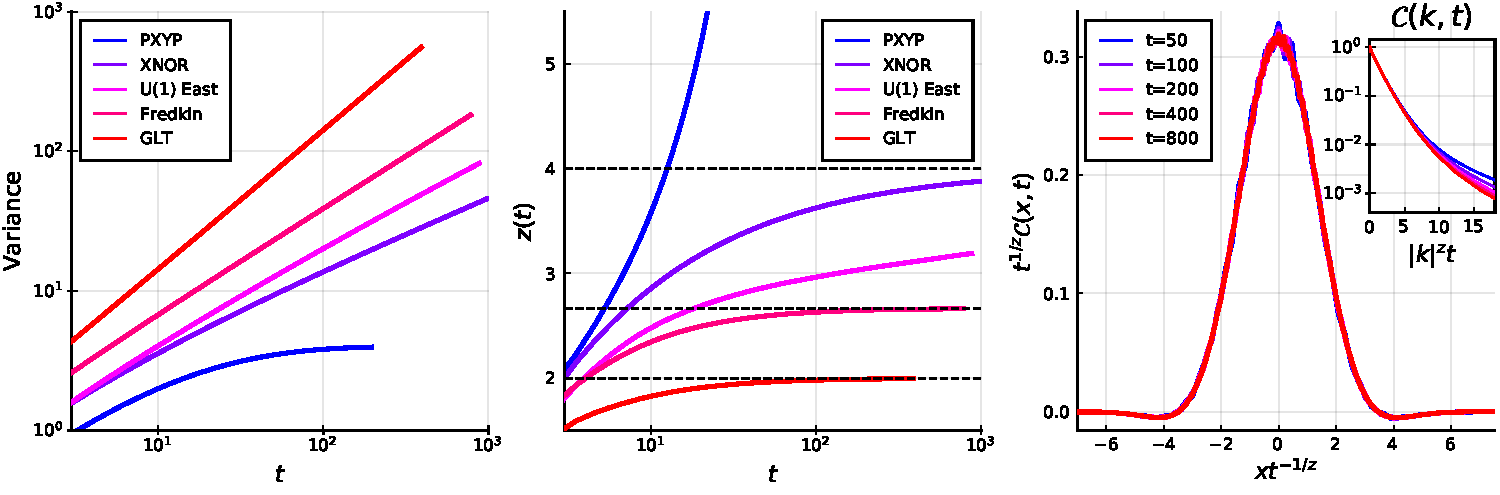
\includegraphics[width=.95\textwidth]{fig2.pdf} 
    \caption{{\bf Numerical results from the transfer matrix, $\Tmat$. }{\it Left}:~Variance of the spin profile in each of the five models. The variance saturates in the PXYP model, indicating localization, while charges eventually spread across the system in the other models. {\it Middle}:~Apparent dynamical exponent, $z$, versus time, $t$. For GLT,  XNOR and Fredkin, $z(t)$ saturates to $z=2$ (diffusion), $z=4$ and $z=8/3$ (subdiffusion), respectively. In the $U(1)$ East model, $z(t)$ appears to grow without bound,  $z(t) \sim \log t$, indicating quasilocalized dynamics with spread slower than any power law --- another way to extract $z(t)$ using the return probability $\Corr (x=0,t) \sim t^{-1/z}$ leads to a different and even larger estimate $z \approx 7$ for the time scales we can access~\cite{supp}.   {\it Right}:~Collapse of charge profiles for Fredkin when rescaled by the dynamical exponent $z=8/3$. {\it Inset}: Collapse in momentum space showing  ${\cal C}(k,t)\sim {\rm e}^{- C |k|^{z} t}$ at small $k$. TEBD data use maximum bond dimension $\chi^{\,}_{\rm max} = 1024$ for Fredkin and $\chi^{\,}_{\rm max} = 512$ for the other models to ensure convergence.
    \label{fig2} }
\end{figure*}
 

\noindent \emph{Two-point correlations.---}\, To compute Haar-averaged two-point functions, we dispense with the ancillary qudit and Floquet structure: The five models considered act on $L$ qubits ($\Ldim=2$) with Haar unitaries independently drawn at each time step. Correlators \eqref{eq:Cdef} in RUCs can generically be written in terms of a transfer matrix, 
\be \label{eq:Cij} \Corr^{\,}_{i,j} = \expval{ \,\overline{\, \observ^{\,}_i (t) \, \observ^{\,}_j (0) \, }\,} = \opmatel{\observ^{\,}_i}{\, \Tmat^{\, t \,}\, }{\observ^{\,}_j}~~,~~\ee
where $\opket{\observ}$ is an element of the $\Ldim^{2L}$-dimensional operator space, and $\Tmat$ acts therein, is implicitly Haar averaged \footnote{Each layer of the transfer matrix can be ensemble averaged independently, as unitary gates are independently drawn at each time step.}, and has the same circuit structure as $\Floq$ (and the SFF transfer matrix). For models with Hilbert space dimension $\Ldim$ and unitaries given by Eq.~\ref{eq:GateForm}, the gates of $\Tmat$ take the form~\cite{supp} $\opmatel{\sigma^{\mu}_r}{\Tgate^{\,}_r }{\sigma^{\nu}_r} \, = \, \Ldim^{-\ell} \, \tr{ \, \sigma^{\mu}_r \, \overline{\, \gate^{\dagger}_{r} \, \sigma^{\nu}_r \gate^{\vpd}_r \,}\,}$,
 where $ \opinprod{\sigma^{\mu}_r}{\sigma^{\nu}_r} = \delta^{\,}_{\mu,\nu}$ are orthonormal basis operators (e.g. Pauli strings for $q=2$). Haar averaging gives 
 %(
\be \label{eq:CorrTGate} \Tgate^{\,}_r  \, = \, \sum\limits_{\alpha} \, \frac{1}{n^{\,}_{\alpha}} \, \sum\limits_{m,m' \, \in \, \alpha \,} \, | \, \pi^{\,}_m )( \pi^{\,}_{m'} |~~,\ee %)
for diagonal (i.e., charge conserving) operators, where $\opket{\pi^{\,}_m} \, = \, \sqrt{\Ldim}\, \ket{m} \bra{m}$ is a projector onto state $m$ in block $\alpha$, and $\opinprod{\pi^{\,}_m}{\pi^{\,}_n} = \delta^{\,}_{m,n}$ form an orthonormal basis for the $\Ldim$ diagonal operators on each site \cite{supp}. 

Crucially, we note that $\Tmat$ \eqref{eq:CorrTGate} is identical to the SFF transfer matrix \eqref{eq:Tgate}, with the $\Ldim$ states per site replaced by $\Ldim$ charge-conserving operators. Thus, the universal features of both spectral and physical correlations are controlled by the low energy spectrum of $\Tmat$, generically relating the Thouless time (related to spectral rigidity) to transport properties, as proposed in Ref.~\citenum{ShenkerRMT}. 
As an aside, we note that nondiagonal (charge-changing) operators do not mix with diagonal operators under $\Tmat$, but evolve under a different transfer matrix if at all \cite{supp}. %Correlators of diagonal (charge) operators are sufficient to extract transport properties, and we now turn to numerical study of $\Tmat$.
However, we need only consider correlators of diagonal (charge) operators to extract universal transport properties.

\noindent \emph{Numerics.---}\, 
We efficiently simulate the dynamics generated by $\Tmat$ using time evolving block decimation (TEBD) applied to matrix-product operators (MPOs)~\cite{PhysRevLett.91.147902,PhysRevLett.93.207204,PhysRevLett.93.040502,SCHOLLWOCK201196}, exploiting slow entanglement growth compared to the underlying unitary dynamics. We simulate infinite-temperature correlation functions $\Corr (x,t) = \, \Hdim^{-1} \, \tr{ \, \overline{ \, \charge (x, t) \, \charge (0,0) \,} \,}$, where $\charge (x,t)$ is the occupation of site $x$ at time $t$. %The explicit form of $\Tgate^{\,}_r$ for each model is provided in Ref.~\citenum{supp}. 
We also use the spatial variance of %$\Corr$'s profile
the correlator,~$\sigma^{2}(t) = \sum_{x} \, x^2 \, \Corr(x,t) - (\sum_{x} \, x \, \Corr(x,t))^{2} \sim t^{2/z}$, to extract
the dynamical exponent, $z$---characterizing the transport of charge---via %a logarithmic derivative 
$2/z(t) \equiv   d \log \sigma^2 / d \log t $ (shown in the center panel of Fig.~\ref{fig2}).
For GLT, $z(t) \to 2$, indicating diffusive transport and consistent with classical results \cite{GLT}; for XNOR and Fredkin, $z=4$ and $z \simeq 8/3$, respectively, indicating subdiffusion; 
for PXYP, $\sigma^{2}(t)$ itself saturates, indicating localization; and for $U(1)$ East, $z(t)$ grows slowly without saturation, indicating %quasilocalized behavior ($\sigma^2(t)$ grows more slowly with time than any power law).
quasilocalization.

The PXYP and $U(1)$ East cases can be understood in terms of {\em Hilbert space fragmentation} \cite{RahulFractonCircuit,RahulShattering,PabloFragmentPRX,moudgalya2019thermalization,SLIOM1,kohlert2021experimental,SLIOM1}: The number of sectors, $\numsec$, for both models scales exponentially in system size~\cite{supp}. In the terminology of Ref.~\citenum{PabloFragmentPRX}, PXYP is ``strongly fragmented'' and does not thermalize (i.e. there is no transport; charges are localized), while $U(1)$ East is ``weakly fragmented'' and thermalizes very slowly ($\sigma^2(t)$ grows more slowly with $t$ than any power law). XNOR also shows weak fragmentation, and its dynamical exponent, $z=4$, can be derived analytically from the unusual spin-wave spectrum, $E(k) \sim k^2/L^2$ of the underlying effective RK Hamiltonian~\cite{supp}. This subdiffusive transport with $z=4$ can also be understood in terms of the ``screening'' of the effective charge carried by the diffusive magnon excitations in this model~\cite{PhysRevLett.122.127202,supp}.

We remark that $z(t)$ appears to approach $8/3$ for Fredkin constraints---a similar numerical estimate, $z \approx 2.69$, was reported in Ref.~\citenum{ChenFredkin2017a} in the context of low-temperature physics of the Fredkin Hamiltonian. While our results derive from RUCs, we expect that this $z=8/3$ characterizes a new dynamical universality class of \emph{generic} many-body quantum or classical systems (Floquet, Hamiltonian, or noisy) with Fredkin constraints. The Fredkin correlator satisfies the universal scaling form $\Corr(x,t) \sim 1/t^{1/z} f(x/t^{1/z})$, with $f(\cdot)$ a non-Gaussian function (see third panel of Fig.~\ref{fig2} and Ref.~\citenum{supp}).  Remarkably, we find numerically that the Fredkin RK Hamiltonian has a low-energy spectrum $E(k) \sim k^{4/3}/L^{4/3}$, reminiscent of the XNOR model, suggesting the possibility of a similar mechanism for subdiffusion in both models~\cite{supp}.


\noindent \emph{Discussion.---}\, 
We studied spectral and transport properties of many-body quantum systems with conserved charges and kinetic constraints using random unitary circuits. We computed ensemble-averaged spectral form factors and linear-response correlation functions for various classes of constraints, and showed that both relate to the same transfer matrix, $\Tmat$, describing a classical Markov process%, or equivalently, an effective Hamiltonian at an RK point. We note that these mappings hold 
. This mapping holds for \emph{any} choice of symmetries and constraints, and in any dimension; however, numerical simulation of $\Tmat$ becomes intractable for $d>1$. Our results establish a general correspondence between the Thouless time and transport properties in conserving systems, and we unearth a broad range of possible transport properties depending on the %choice of constraints. 
constraint. The Fredkin universality class is especially interesting: Further characterizing its dynamical exponent of $z \simeq 8/3$ presents a clear direction for future work. 


\noindent \emph{Acknowledgments.---}\, %We acknowledge useful discussions and related collaborations with U. Agrawal, J. T. Chalker, A. De Luca, and A.C. Potter, as well as J. P. Garrahan, S. Gopalakrishnan, A. Lucas, R. Nandkishore, B. Pozsgay, T. Rakovszky, P. Sala, and W. Witczak-Krempa, whom we also thank for feedback on this manuscript. We acknowledge support from the Air  Force  Office  of  Scientific  Research  under  Grant No. FA9550-21-1-0123  (RV and BAW) and the Alfred P. Sloan Foundation through a Sloan Research Fellowship (RV).
We thank U. Agrawal, J. T. Chalker, A. De Luca, and A.C. Potter for useful discussions and collaborations on related work; we thank J. P. Garrahan, S. Gopalakrishnan, A. Lucas, R. Nandkishore, B. Pozsgay, T. Rakovszky, P. Sala, and W. Witczak-Krempa for the same and for their feedback on this manuscript. We acknowledge support from the Air  Force  Office  of  Scientific  Research  under  Grant No. FA9550-21-1-0123  (RV and BAW) and the Alfred P. Sloan Foundation through a Sloan Research Fellowship (RV).

\noindent {\it Note Added.---}\, While completing this manuscript, Ref.~\citenum{Pal2021Motzkin} appeared on the arXiv, and reports subdiffusive hydrodynamics for the ``Motzkin'' Hamiltonian; Motzkin constraints are very similar to Fredkin constraints, and appear to lie in the same universality class with dynamical exponent $z\simeq 8/3$~\cite{supp}.




\bibliography{RUFC}


\bigskip

\onecolumngrid
\newpage

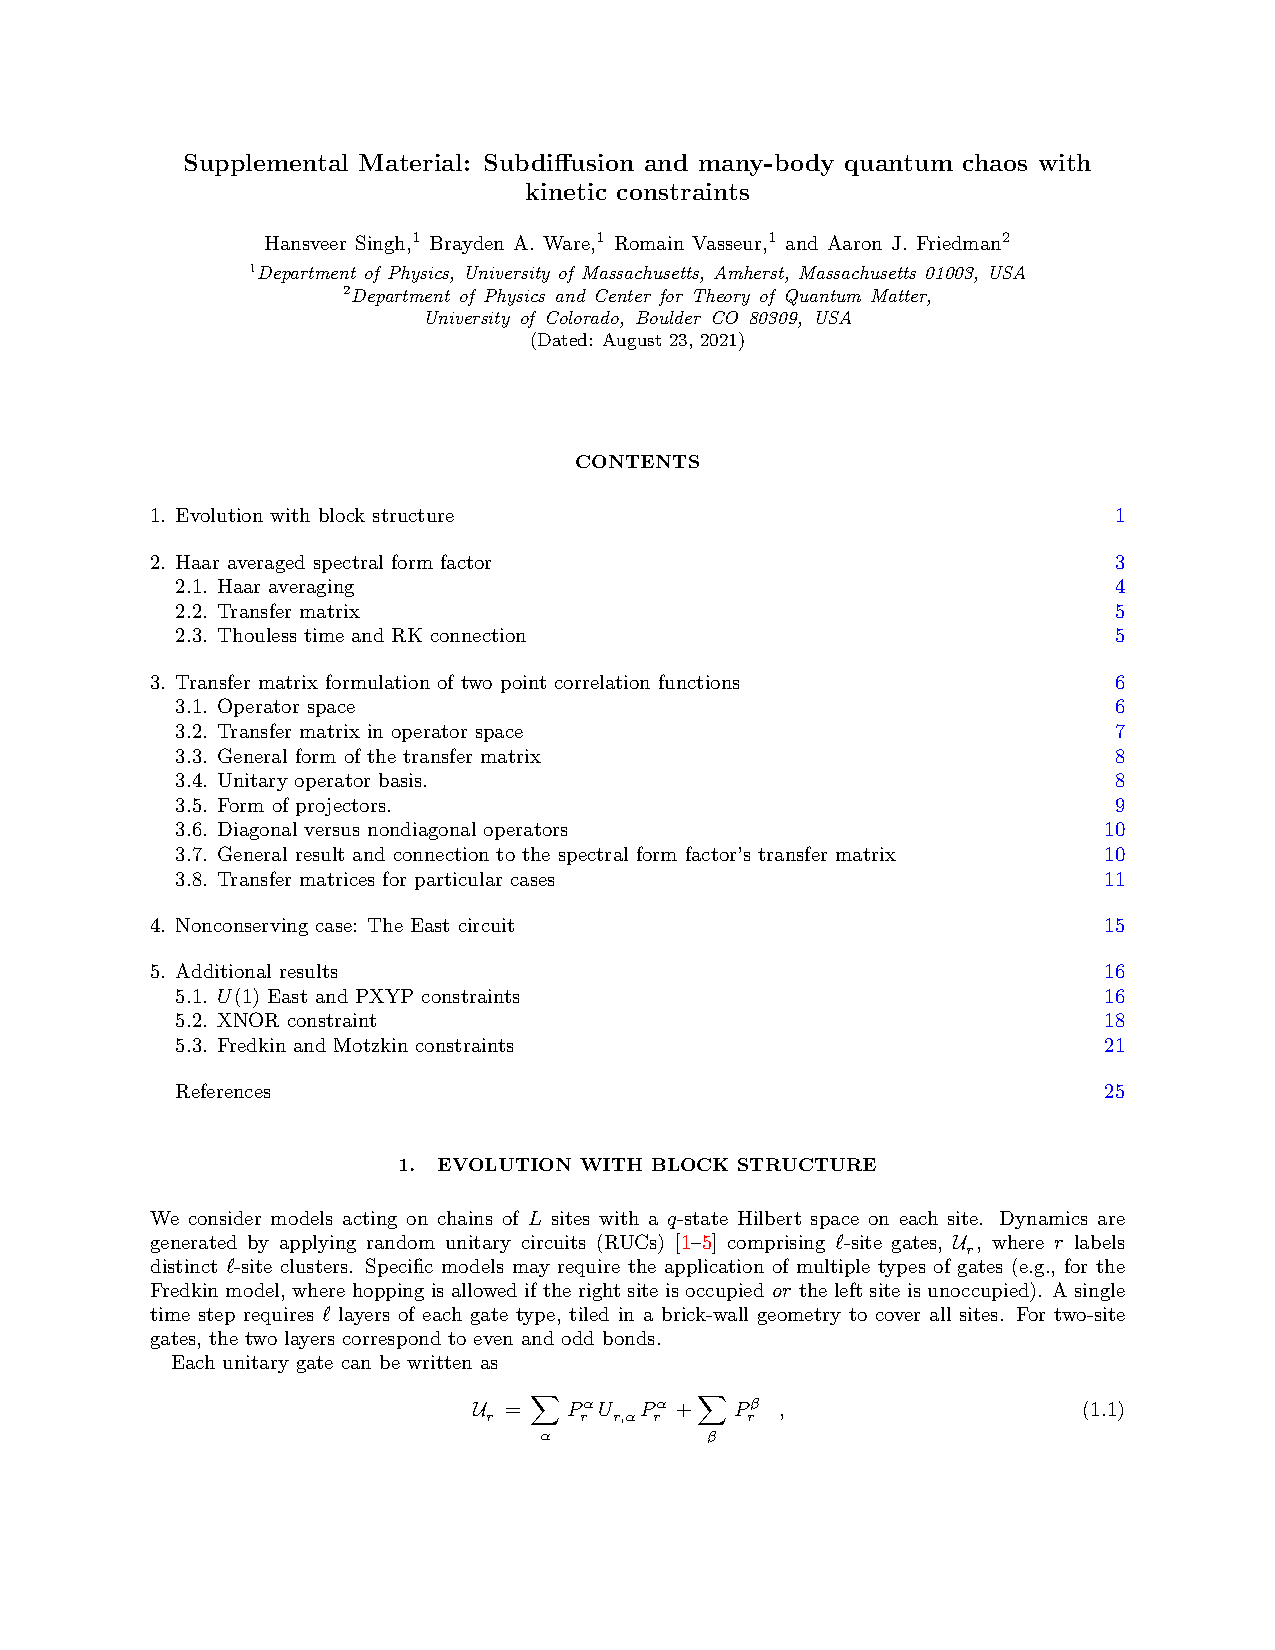
\includepdf[pages=1]{supplement.pdf}
\newpage
\includepdf[pages=2]{supplement.pdf}
\newpage
\includepdf[pages=3]{supplement.pdf}
\newpage
\includepdf[pages=4]{supplement.pdf}
\newpage
\includepdf[pages=5]{supplement.pdf}
\newpage
\includepdf[pages=6]{supplement.pdf}
\newpage
\includepdf[pages=7]{supplement.pdf}
\newpage
\includepdf[pages=8]{supplement.pdf}
\newpage
\includepdf[pages=9]{supplement.pdf}
\newpage
\includepdf[pages=10]{supplement.pdf}
\newpage
\includepdf[pages=11]{supplement.pdf}
\newpage
\includepdf[pages=12]{supplement.pdf}
\newpage
\includepdf[pages=13]{supplement.pdf}
\newpage
\includepdf[pages=14]{supplement.pdf}
\newpage
\includepdf[pages=15]{supplement.pdf}
\newpage
\includepdf[pages=16]{supplement.pdf}
\newpage
\includepdf[pages=17]{supplement.pdf}
\newpage
\includepdf[pages=18]{supplement.pdf}
\newpage
\includepdf[pages=19]{supplement.pdf}
\newpage
\includepdf[pages=20]{supplement.pdf}
\newpage
\includepdf[pages=21]{supplement.pdf}
\newpage
\includepdf[pages=22]{supplement.pdf}
\newpage
\includepdf[pages=23]{supplement.pdf}
\newpage
\includepdf[pages=24]{supplement.pdf}
\newpage
\includepdf[pages=25]{supplement.pdf}
\newpage
\includepdf[pages=26]{supplement.pdf}

\end{document}






\end{document}

